\section{Recurrent and Graph Neural Networks}
\subsection{Backpropagation through time}
\begin{itemize}
	\item Sequences are of arbitrary length. Standard networks like CNN mostly work on fixed input dimensionality
	\item Usage of memory with shared weights $\theta$: $$c_{t+1} = h_{\theta}\left(x_{t+1}, c_{t}\right) = h_{\theta}\left(x_{t+1}, h_{\theta}\left(x_{t}, c_{t-1}\right)\right) = ...$$
	\item Simple RNN cell: 
	\begin{equation*}
		\begin{split}
			c_t & = \tanh\left(U\cdot x_t + W \cdot c_{t-1}\right) \\
			y_t & = \text{softmax}\left(V \cdot c_{t}\right) \\
			\loss & = \sum\limits_{t=1}^{T} y_t^{*} \log y_t \\
		\end{split}
	\end{equation*}
	\item Gradient for output weights $V$:
	\begin{equation*}
		\begin{split}
			\pd{\loss_t}{V} & = \chain{\loss_t}{y_t}{c_t}\pd{c_t}{V} = \left(y_t - y_t^{*}\right) \cdot \left(c_t\right)^T\\
			\pd{\loss}{V} & = \sum\limits_{t=1}^{T} \pd{\loss_t}{V}\\
		\end{split}
	\end{equation*}
	\item Gradient for memory weights $W$: 
	\begin{equation*}
		\begin{split}
			\pd{\loss_t}{W} & = \chain{\loss_t}{y_t}{c_t}\pd{c_t}{W}\\
		\end{split}
	\end{equation*}
	\begin{itemize}
		\item In $\pd{c_t}{W}$, $c_t$ depends on $c_{t-1}$ which again depends on $W$. Thus, we have a recurrence in the gradient calculation:
		$$\pd{\loss_t}{W} = \sum\limits_{k=1}^{t} \chain{\loss_t}{y_t}{c_t}\chain{c_t}{c_k}{W}$$
		where $\pd{c_k}{W}$ only models the dependency exactly at time step $k$
		\item The gradient $\pd{c_t}{c_k}$ can be determined by the chain rule: $\pd{c_t}{c_k} = \prod\limits_{i=k+1}^{t} \pd{c_i}{c_{i-1}}$
		\item All in all, the final loss is:
		\begin{equation*}
			\begin{split}
				\pd{\loss}{W} & = \sum\limits_{t=1}^{T}\sum\limits_{k=1}^{t} \chain{\loss_t}{y_t}{c_t}\left(\prod\limits_{i=k+1}^{t} \pd{c_i}{c_{i-1}}\right)\pd{c_k}{W}
			\end{split}
		\end{equation*}
	\end{itemize}
	\item Gradient for input weights $U$ very similar to $W$: 
	\begin{equation*}
		\begin{split}
			\pd{\loss}{U} & = \sum\limits_{t=1}^{T}\sum\limits_{k=1}^{t} \chain{\loss_t}{y_t}{c_t}\left(\prod\limits_{i=k+1}^{t} \pd{c_i}{c_{i-1}}\right)\pd{c_k}{U}
		\end{split}
	\end{equation*}
	\item The problem with RNNs are that the gradients at time step $t$ depend on $c_{t-1}$ which also depends on $w$. However, the gradients are calculated with the assumption that $w$ stays the same for the previous time steps.
	\item This error can easily accumulate over many time steps so that in very long sequences, the gradients for the last steps are inaccurate
	\item Reduce learning rate/fewer updates, but this leads to slower training
\end{itemize}
\subsubsection{Vanishing gradients}
\begin{itemize}
	\item The exact derivations can be found in \href{http://proceedings.mlr.press/v28/pascanu13.pdf}{this paper}
	\item We assume an alternative formulation for simplicity here: $c_t = W \cdot \sigma(c_{t-1}) + U \cdot x_{t-1}$ where $\sigma$ is an arbitrary activation function. Then, the partial derivative between two time steps is\\ $\pd{c_{t}}{c_{k}} = \prod\limits_{i=k+1}^{t} \pd{c_{i}}{c_{i-1}} = \prod\limits_{i=k+1}^{t} W^T \cdot \text{diag}\left(\pd{\sigma\left(c_t\right)}{c_t}\right)$
	\item Hence, the magnitude of $\pd{c_{t+1}}{c_{t}}$ is bounded by this derivative: 
	$$\left\lVert \pd{c_{t+1}}{c_{t}}\right\rVert \leq \left\lVert W^T\right\rVert \cdot \left\lVert \text{diag}\left(\pd{\sigma\left(c_t\right)}{c_t}\right)\right\rVert$$
	\item In case the derivative of our non-linearity is bounded to a value $\gamma$ (which is 1 in case of tanh), we know that gradients vanish if the norm of the weight gradients are lower than $1/\gamma$:
	$$\left\lVert \pd{c_{t+1}}{c_{t}}\right\rVert \leq \left\lVert W^T\right\rVert \cdot \left\lVert \text{diag}\left(\pd{\sigma\left(c_t\right)}{c_t}\right)\right\rVert < \frac{1}{\gamma}\gamma = 1$$
	\item This term is exponentiated with the number of time steps. Thus, long sequences suffer even more of vanishing gradients $\Rightarrow$ learn only short-term relationships
	\item If however $\left\lVert \pd{c_{t+1}}{c_{t}}\right\rVert > 1$ because of $\left\lVert W^T\right\rVert \gg 1/\gamma$, then we can get exploding gradients
	\item Quick fix for exploding gradients: clip gradient norm. However, there the counterpart can happen where we only focus on long-term relationships
\end{itemize}
\subsubsection{Long Short-Term Memory}
\begin{itemize}
	\item Preventing vanishing gradients by gate mechanism
	\item By simply adding features to memory and limiting memory by sigmoid we can get strong gradients for any sequence length. Note that the gradients get lower in expectation because sigmoid has mean $0.5$. Nevertheless, if long-term dependencies are important, the network can learn them now
	\item \textit{Forget gate}: regulating how much information is kept from last time step
	\item \textit{Input + candidate gate}: Regulating which, and how much new information should be added given the current time step
	\item \textit{Output gate}: What features are important for the current time step
	\begin{figure}[ht!]
		\centering
		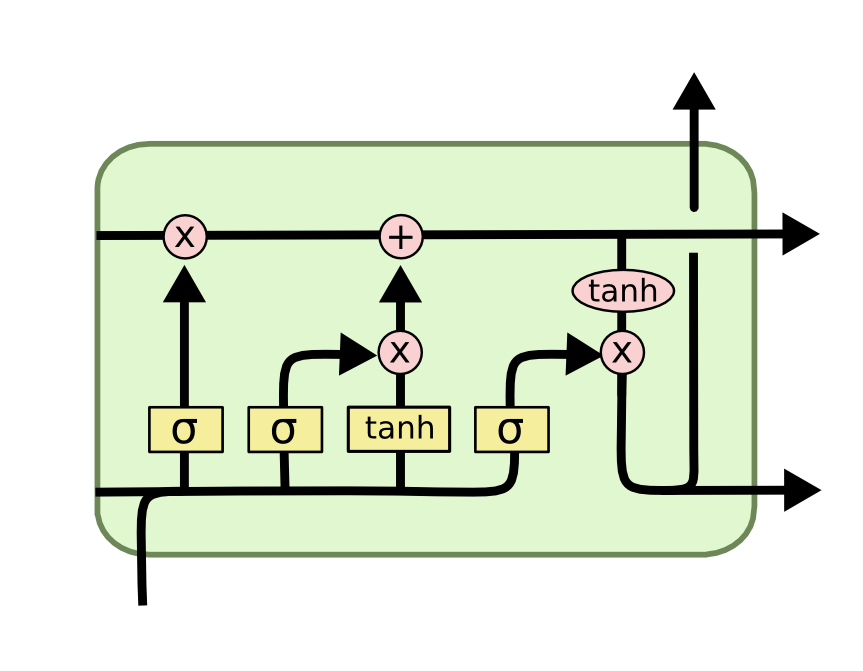
\includegraphics[width=0.3\textwidth]{figures/RNN_LSTM.png}
		\caption{Visualization of a LSTM cell}
		\label{fig:RNN_LSTM}
	\end{figure}
\end{itemize}
\subsection{Graph Neural Networks}
\begin{itemize}
	\item Perform operation on graph-structured data (e.g. social networks or knowledge graphs)
\end{itemize}
\subsubsection{Deep Walk}
\begin{itemize}
	\item Learning latent representations of vertices in a network
	\item The Deep Walk algorithm consists of two simple steps:
	\begin{enumerate}
		\item Perform random walks on the graph to generate node sequences
		\item Run skip-gram on sequence (with word window) to learn node embeddings
	\end{enumerate}
	\item \textit{Drawback}: algorithm has to be re-run if a new node is added, not useful for dynamic graphs
\end{itemize}
\subsubsection{GraphSage}
\begin{itemize}
	\item In every iteration, aggregate information of neighbors and the node itself to generate new embeddings
	\item Aggregation techniques are taking the mean (with weight and non-linearity applied on it afterwards), max pooling, or using a LSTM
\end{itemize}
\subsubsection{Graph Convolutional Networks}
\begin{itemize}
	\item A GNN layer takes as input the embeddings for every node $H^{(l)}$ and the adjacency matrix $A$, and create new embeddings $H^{(l+1)}$
	\item Graph convolutional layers use for this a matrix multiplication where weights are shared over nodes
	\item In the simplest form, a GCN layer can be defined as $h(H^{(l)}, A) = \sigma\left(A H^{(l)} W^{(l)}\right)$
	\item To make it more efficient, we add the identity matrix to $\hat{A} = A + I$ so that nodes use their old embeddings as well, and take the mean instead of the sum over all neighbors (by degree matrix $D$):
	$$h(H^{(l)}, A) = \sigma\left(D^{-1/2}\hat{A}D^{-1/2} H^{(l)} W^{(l)}\right)$$
\end{itemize}